\chapter{Tabular models} \label{ch:tabular}
\begin{NoteBox}
At present we allow only three independent variables in \Vaango.
\end{NoteBox}

MPM tabular material data is often of the form  shown in Figure~\ref{fig:tabular_data}.
In this particular data set, we have three independent variables: the plastic strain ($\beta$),
the saturation ($\alpha$), and the strain ($\Veps$).  Pressure ($p$) is the dependent variable.
The data represents a function of the form $p = p(\Veps, \alpha, \beta)$.  We are given 
an input point in the three-dimensional independent variable space, 
($\Veps_0$, $\alpha_0$, $\beta_0$), and we would like to find the corresponding value of
the pressure, $p_0$.
\begin{figure}[htbp!]
  \centering
  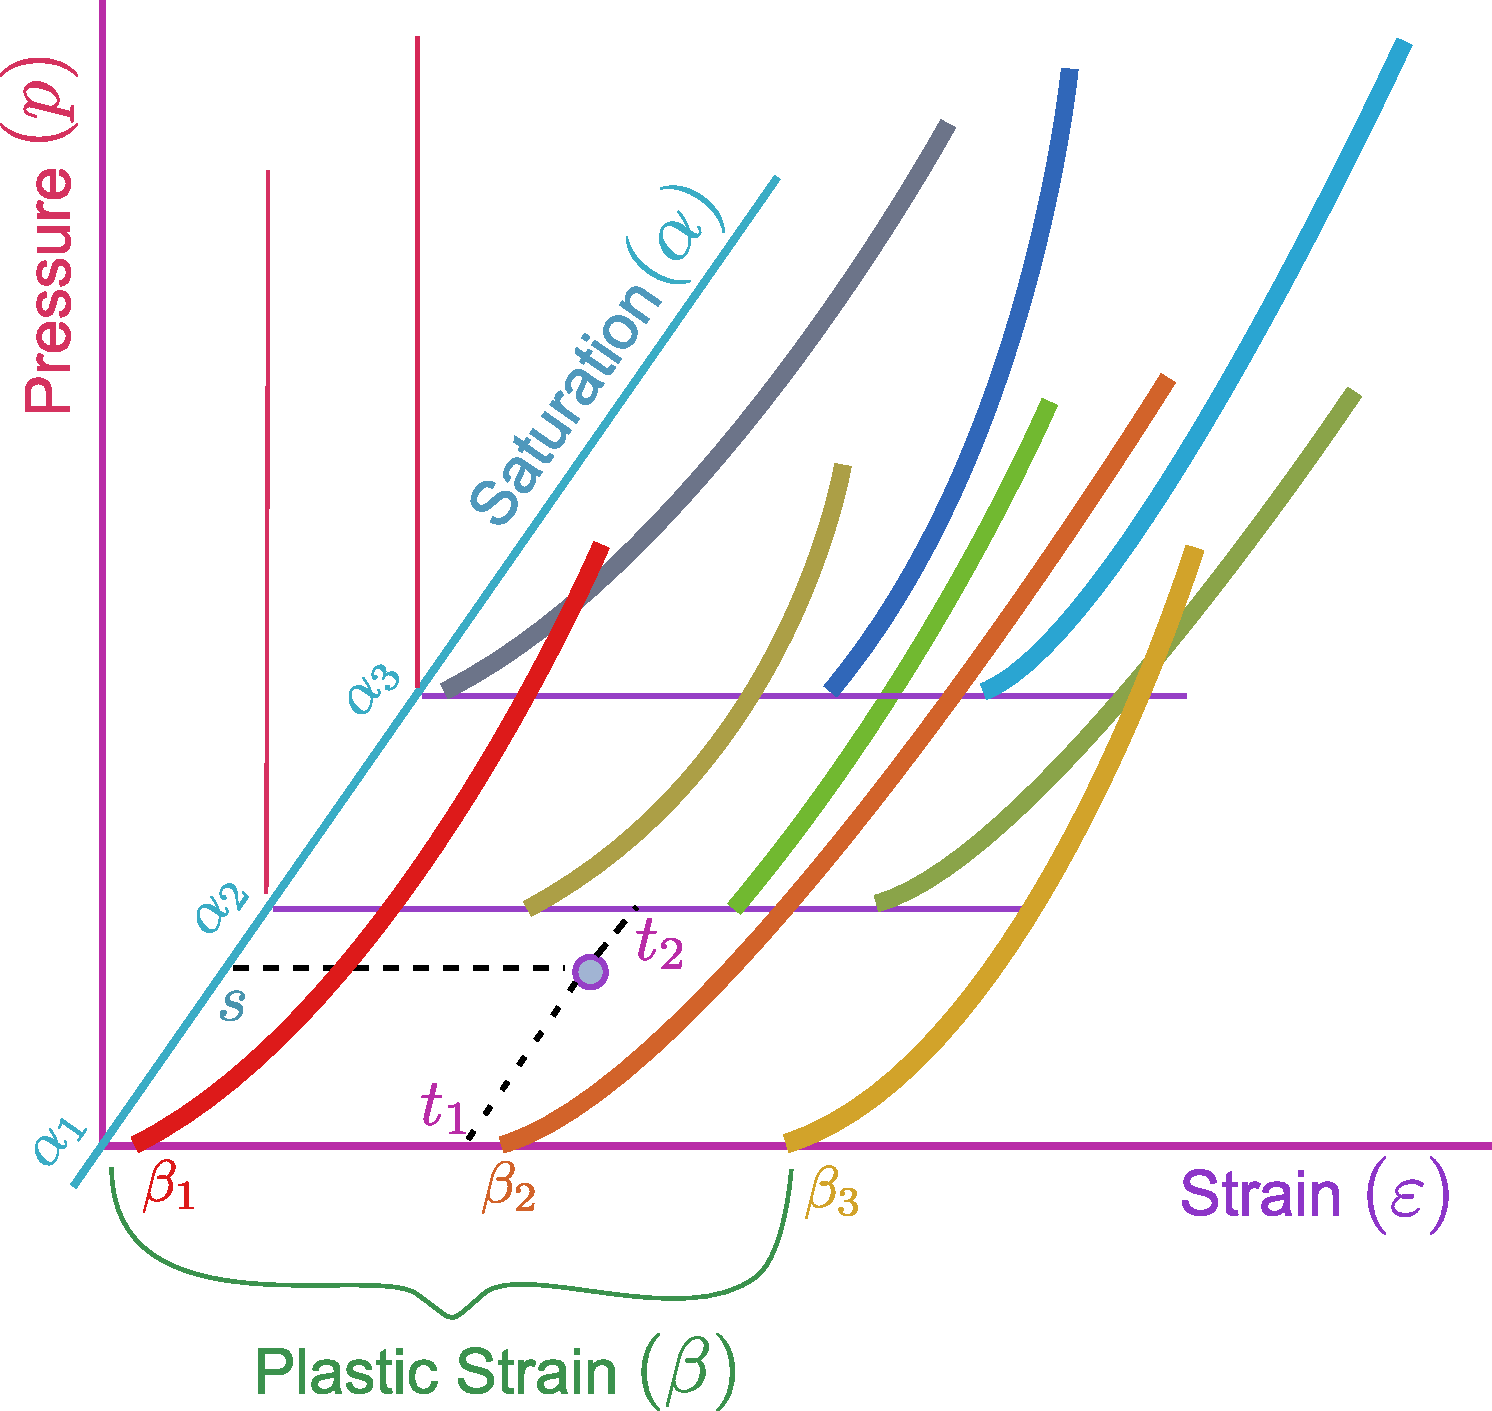
\includegraphics[width=0.5\textwidth]{Figs/tabular/table_interpolation.pdf}
  \caption{Schematic of tabular material data for MPM constitutive models. The circle
           in blue is the input data point for which we would like to find the pressure.}
  \label{fig:tabular_data}
\end{figure}

As we can see from the figure, the data are largely unstructured.  However, there is
some structure to the data.  For instance, the data are provided for three values of
saturation, $[\alpha_1, \alpha_2, \alpha_3]$.  For each value of $\alpha$, we have 
data for a few plastic strain values: $\alpha_1$ : $[\beta_{11}, \beta_{12}, \beta_{13}]$,
$\alpha_2$ : $[\beta_{21}, \beta_{22}, \beta_{23}, \beta_{24}, \dots]$, and
$\alpha_3$ : $[\beta_{31}, \beta_{32}, \dots]$.  Finally, for each value of the plastic
strain, we have a pressure-strain curve, for example, for
$\alpha_1, \beta_{11}$ : $[\Veps_{111}, \Veps_{112}, \Veps_{113}, \dots, \Veps_{11N}]$ and
$[p_{111}, p_{112}, p_{113}, \dots, p_{11N}]$, or for
$\alpha_3, \beta_{32}$ : $[\Veps_{321}, \Veps_{322}, \Veps_{323}, \dots, \Veps_{32M}]$ and
$[p_{321}, p_{321}, p_{321}, \dots, p_{32M}]$.  Clearly, the data become quite complex
as the number of dimensions is increased.  


\section{Linear interpolation}
\begin{NoteBox}
The procedure below assumes that the $\alpha$ values are sorted in ascending order.
If $\alpha_0 \notin [\alpha_1, \alpha_N]$, \Vaango will throw an exception and
exit.  Also observe that at least two sets of data are needed for the interpolation
procedure to work.
\end{NoteBox}

In this section we describe the process used in \Vaango to interpolate the data.
For simplicity, we only consider two independent variables, the saturation ($\alpha$)
and the strain ($\Veps$) as shown in Figure~\ref{fig:tabular_data_step1}.  
\begin{figure}[htbp!]
  \centering
  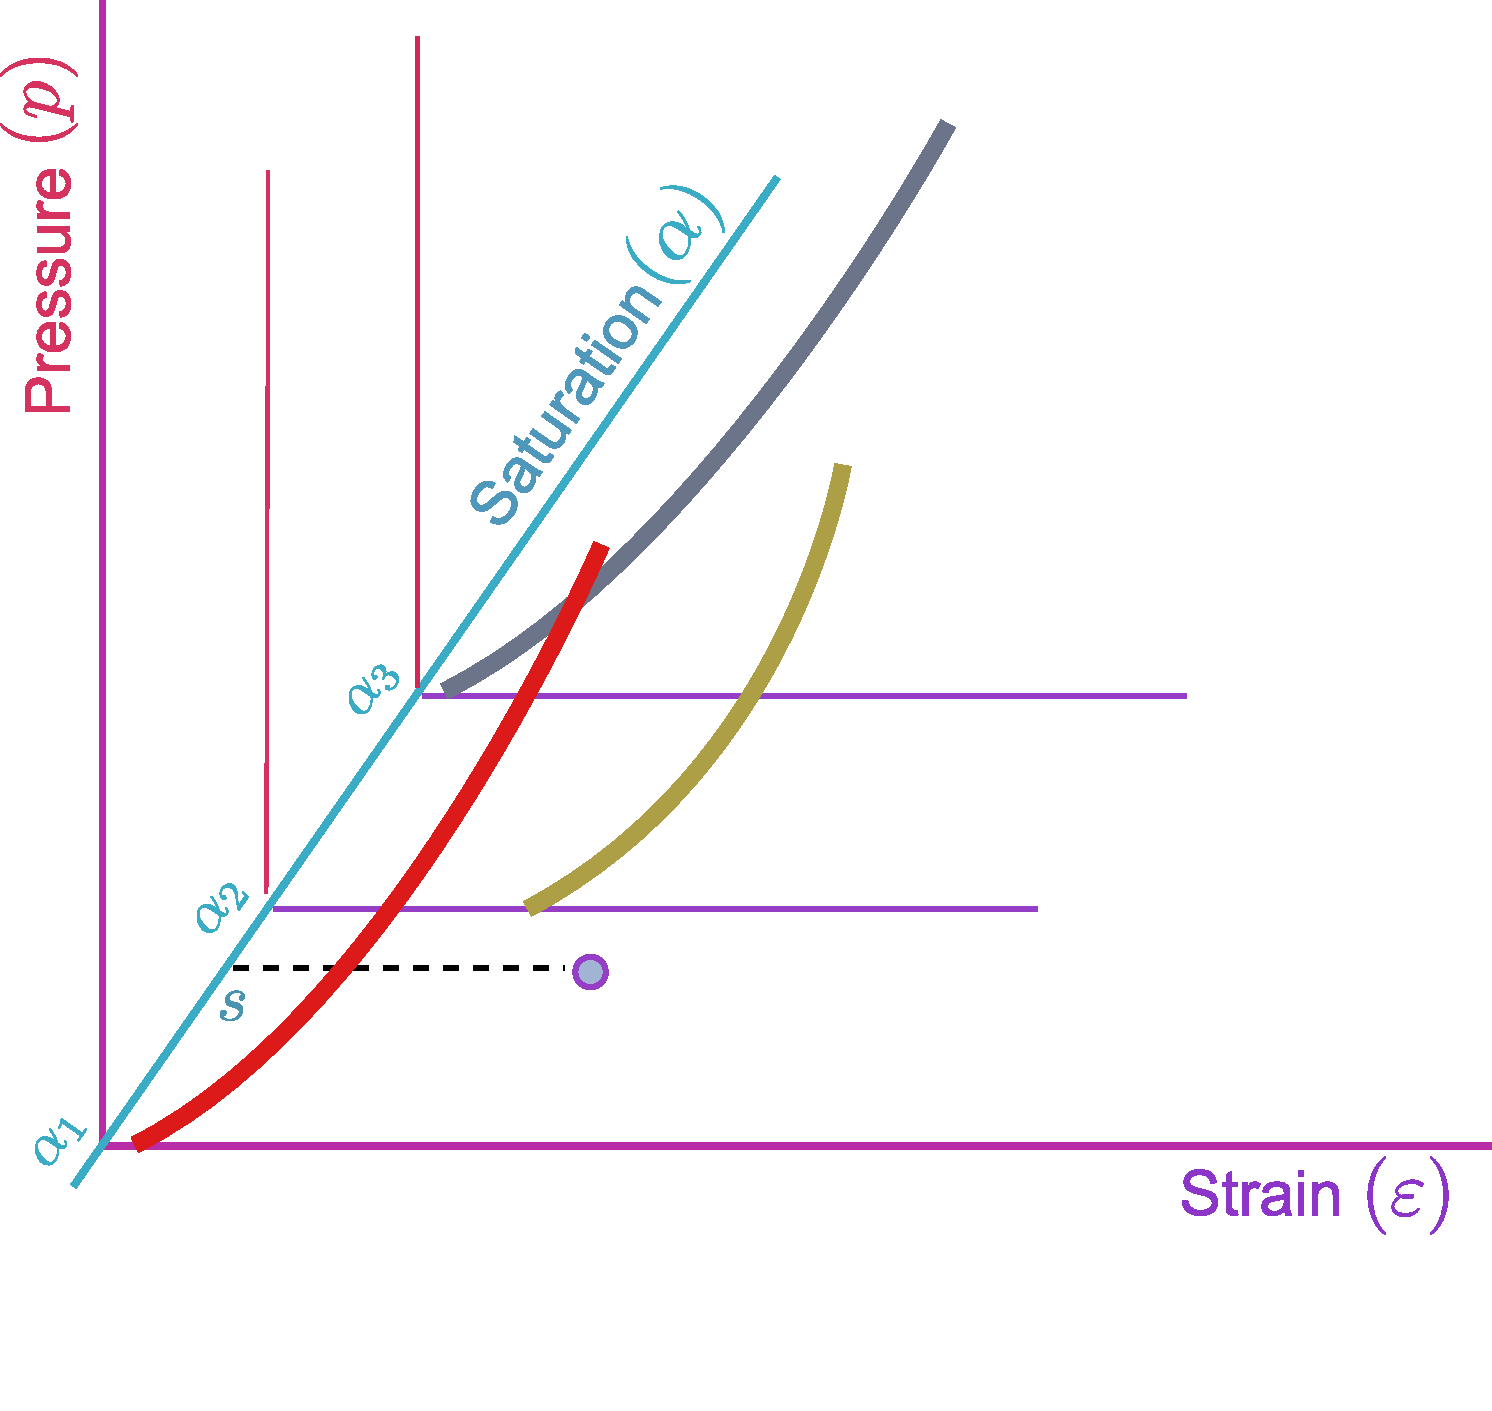
\includegraphics[width=0.5\textwidth]{Figs/tabular/table_interpolation_step1.pdf}
  \caption{Schematic of a three variable table of material data. The 
           circle in blue is the input point for which we would like to find the pressure.}
  \label{fig:tabular_data_step1}
\end{figure}

The first step in the process is to find the pressure-strain data that are needed 
for the interpolation process.  This can be accomplished by iterating through 
the $\alpha$s and finding a value of the parameter $s \in [0,1]$ where
\Beq
  s = \frac{\alpha_0 - \alpha_k}{\alpha_{k+1} - \alpha_k}~,~~ k=1,2,\dots,N-1
\Eeq
where $N$ is the number of values of $\alpha$ for which data area available.


Once the two curves needed for interpolation have been identified, the next step is
to find the segments of the pressure-strain curves that correspond to the input
variable $\Veps_0$.  These segments are highlighted with thick lines in 
Figure~\ref{fig:tabular_data_step2}.  The two associated parameters $t_1$ and $t_2$
are calculated using
\Beq
  \Bal
  t_1 &= \frac{\Veps_0 - \Veps_{j,k}}{\Veps_{j,k+1} - \Veps_{j,k}}~,~~ k=1,2,\dots,M_j-1 \\
  t_2 &= \frac{\Veps_0 - \Veps_{j+1,k}}{\Veps_{j+1,k+1} - \Veps_{j+1,k}}~,~~ k=1,2,\dots,M_{j+1}-1
  \Eal
\Eeq
where $\Veps_{j,k}$ is a point on the pressure-strain curve for saturation $\alpha_j$, 
and $M_j$ is the number of points on the curve.
\begin{figure}[htbp!]
  \centering
  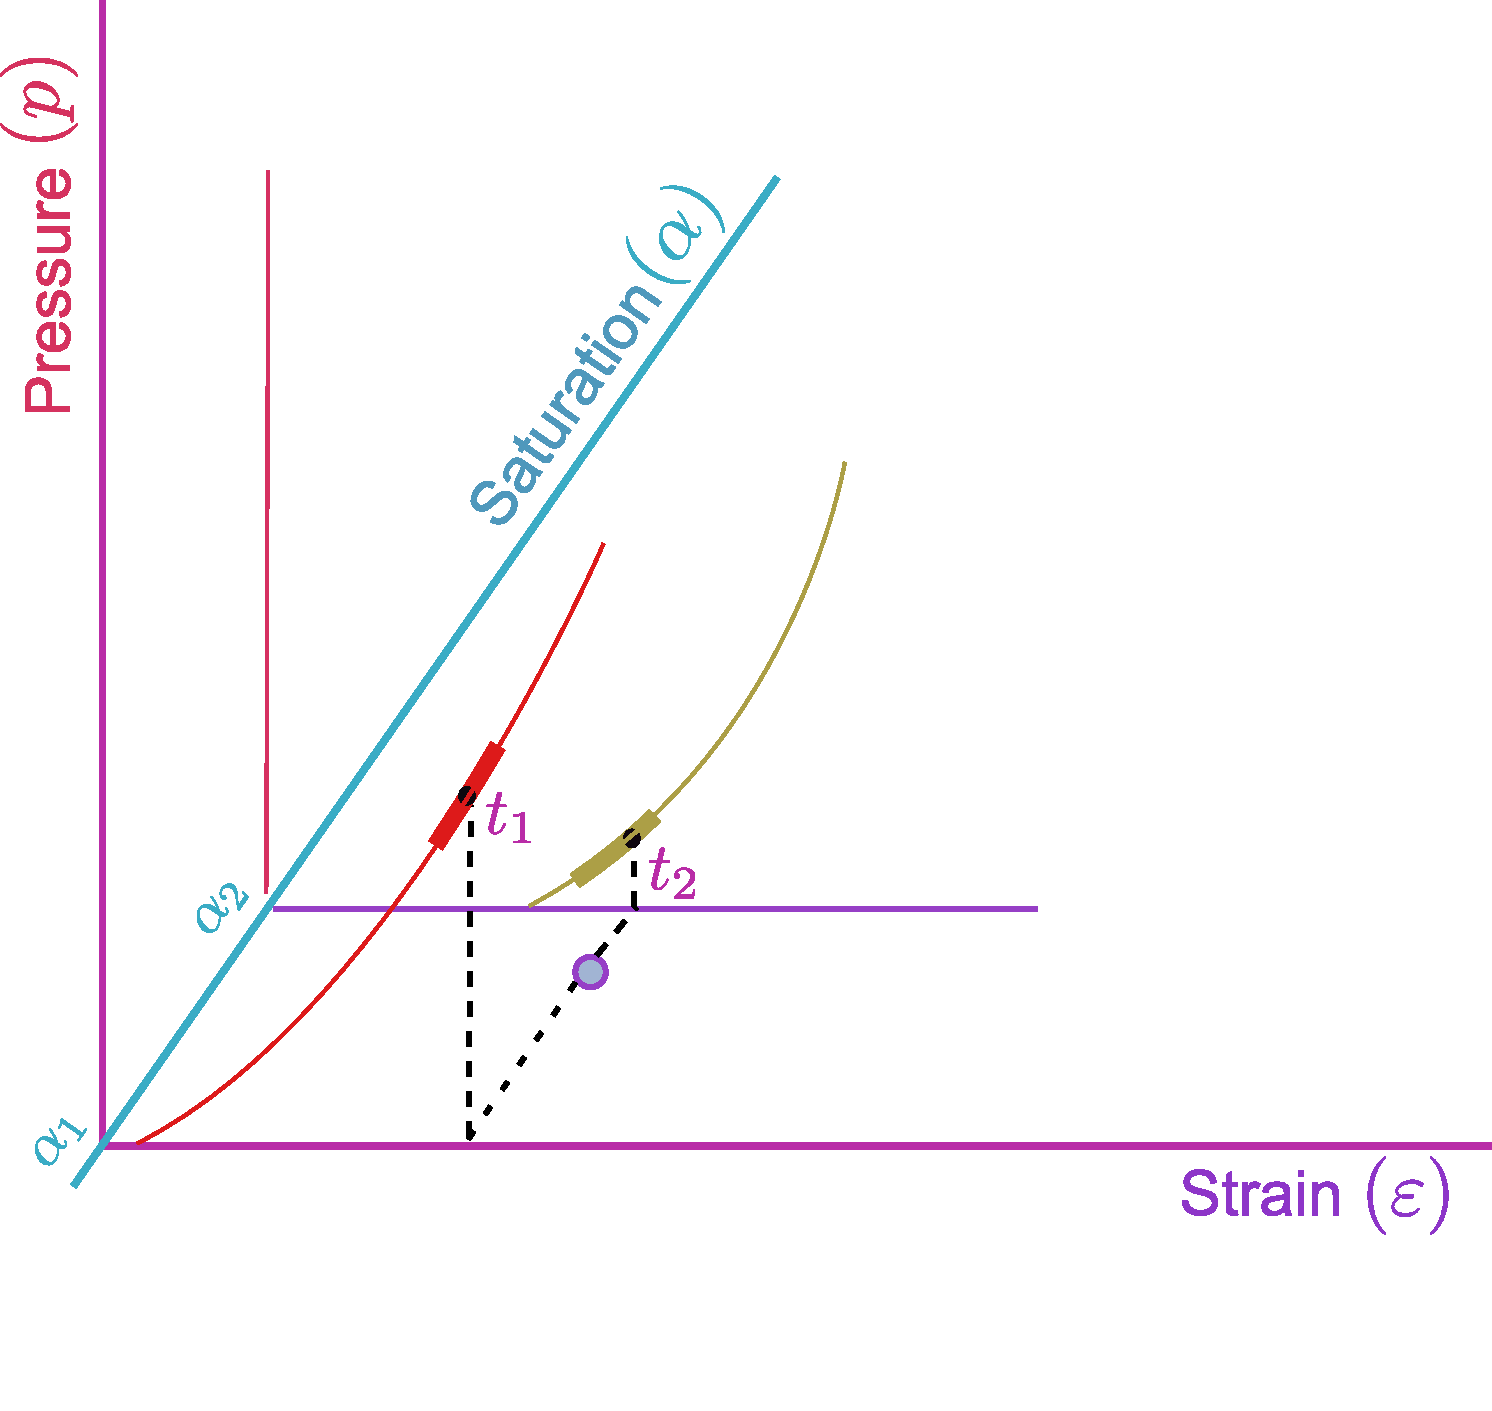
\includegraphics[width=0.5\textwidth]{Figs/tabular/table_interpolation_step2.pdf}
  \caption{Second stage of interpolation of a three variable table of material data. The 
           circle in blue is the input point for which we would like to find the pressure.}
  \label{fig:tabular_data_step2}
\end{figure}

We can now compute the pressures at these two points, using
\Beq
  \Bal
    p_1 &= (1 - t_1) p_{j,k} + t_1 p_{j,k+1} \\
    p_2 &= (1 - t_2) p_{j+1,k} + t_2 p_{j+1,k+1}
  \Eal
\Eeq
The final step of the process is to compute the interpolated pressure $p_0$ using
\Beq
  p_0 = (1 - s) p_1 + s p_2 \,.
\Eeq
A schematic of this operation is shown in Figure~\ref{fig:tabular_data_step3}.
\begin{figure}[htbp!]
  \centering
  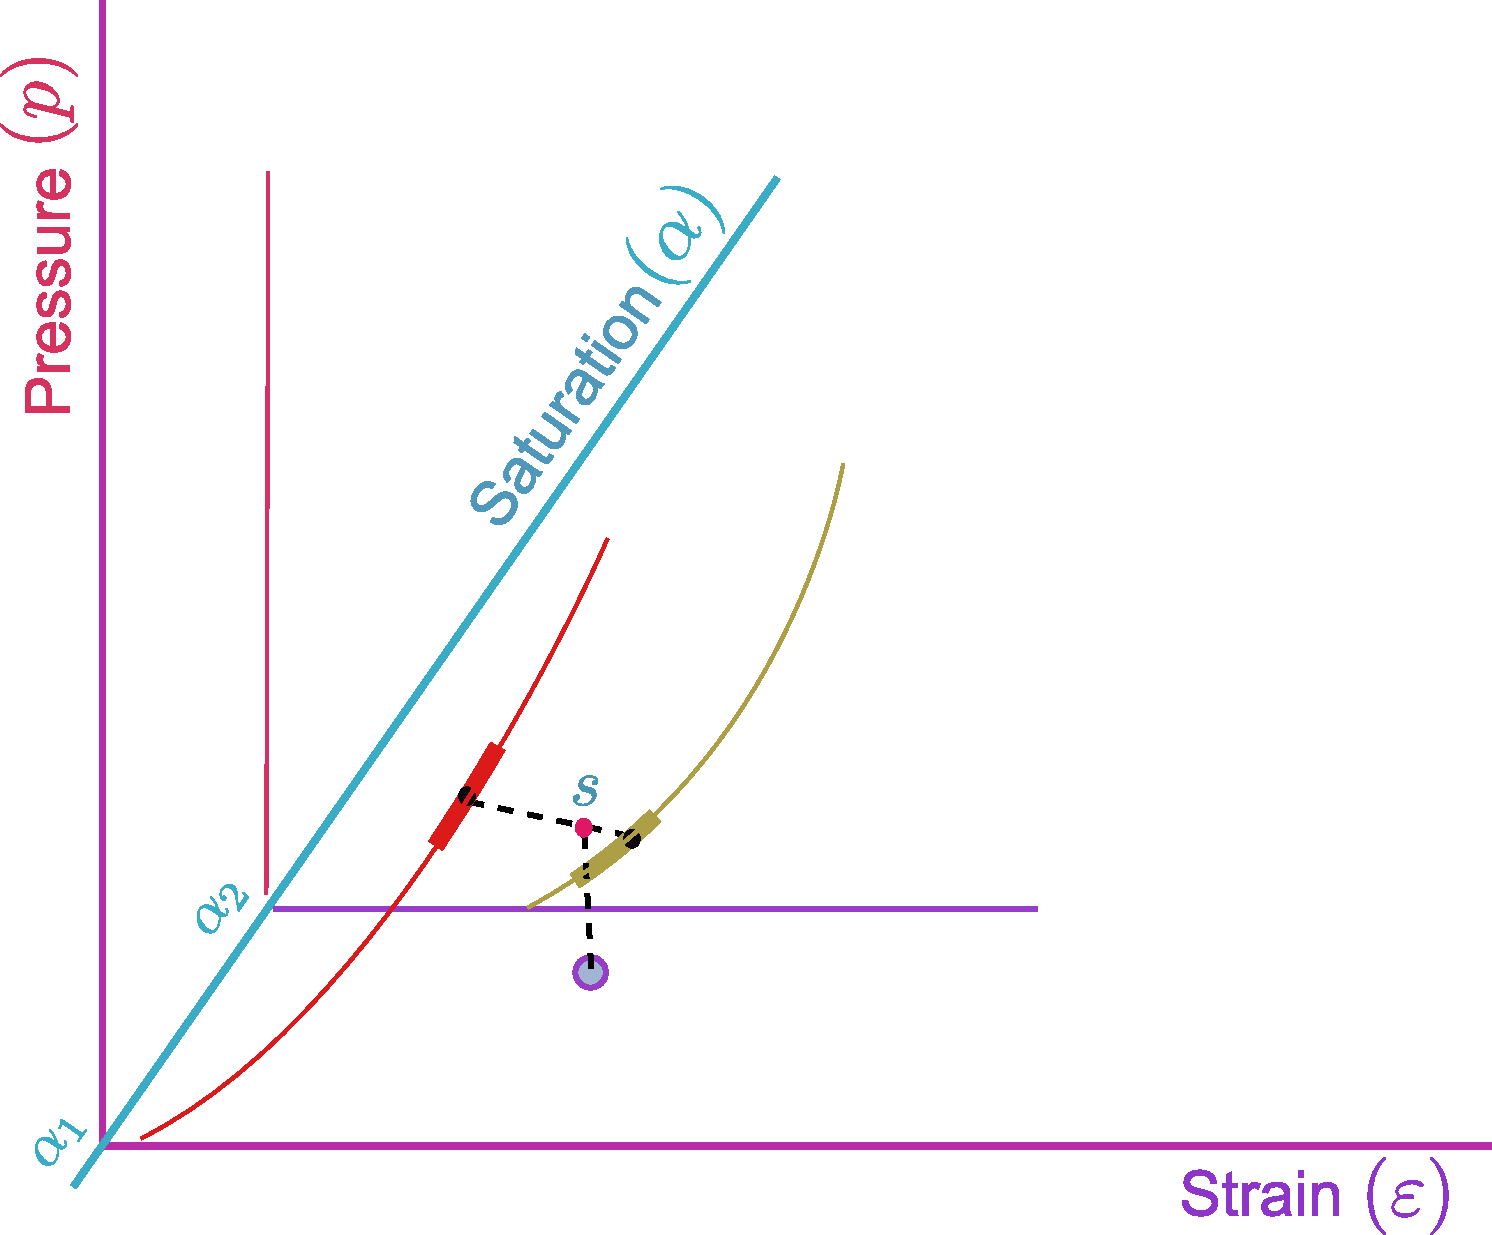
\includegraphics[width=0.5\textwidth]{Figs/tabular/table_interpolation_step3.pdf}
  \caption{Final stage of interpolation of a three variable table of material data. The 
           circle in blue is the input point and the red circle is the interpolated value.}
  \label{fig:tabular_data_step3}
\end{figure}

\section{The tabular equation of state}
For the tabular equation of state, we assume that there is only one independent variable,
the density ratio $\eta = \rho/\rho_0$ where $\rho$ is the current mass density and $\rho_0$ is
its reference value.  The dependent variable is the pressure, $\pbar = \pbar(\eta)$, which is
positive in compression.  A linear interpolation is done to compute the pressure
for a given state of deformation.

The bulk modulus is computed using
\Beq
  K = \rho \left[\frac{p(\eta +\epsilon) - p(\eta-\epsilon)}{2\epsilon}\right]
\Eeq
\begin{WarningBox}
The tolerance $\epsilon$ is hardcoded to $10^{-6}$ in \Vaango but
may not be adequate for some problems.
\end{WarningBox}

